\documentclass[10pt,a4paper,twocolumn]{ltjsarticle}

\usepackage[top=22mm,bottom=24mm,left=18mm,right=18mm]{geometry}
\usepackage{amsmath,amssymb}
\usepackage{booktabs}
\usepackage{graphicx}
\usepackage{enumitem}
\usepackage[hidelinks]{hyperref}

\setlength{\columnsep}{8mm}
\setlength{\parindent}{1em}
\setlength{\parskip}{0pt}

\title{\vspace{-8mm}\bfseries 自分の鎖骨を印刷したい}
\author{
  山名琢翔$^{1}$\\[1mm]
  \small $^{1}$筑波大学大学院 デザイン学学位プログラム 博士前期課程2年\\
  \small \texttt{yamana.takuto.rg@alumni.tsukuba.ac.jp}
}
\date{}

\begin{document}

\twocolumn[
  \maketitle
  \begin{abstract}
    本稿では、CTデータから3Dモデルを作成し、3Dプリンタによって印刷する方法を紹介する。著者は2026年7月に自転車で転倒し右鎖骨を骨折し、病院でCTを撮った。退院後、そのときの画像を入手し、オープンソースソフトウェアによって3Dモデル化した。さらに、3Dモデルを加工し、骨片をつなぐヒンジをつけることで、骨折と整復を体験できる立体パズルを作成した。
  \end{abstract}

  \vspace{1mm}
  \noindent\textbf{Keywords:}
  CT, 3Dモデル, 3Dプリント, 骨折, 鎖骨

  \vspace{5mm}
]

\section{はじめに}

2026年7月、著者は輪行旅\footnote{自分の自転車を交通機関で運び、旅行先で乗ること}の最中、落車した。旅行中は雨の日が多く、雨が止んだタイミングで自転車に乗っていたところ、ブレーキをかけたときに濡れた路面でスリップした。自転車でスリップした場合、自転車と共に倒れると腕や膝をひどく擦りむいてしまうため、私は自転車を離れ、前回り受け身を行った。その際、首から下げていたサングラスを首と右鎖骨の間に挟み、その状態で強い衝撃がかかった結果、右鎖骨を骨折した。落車後すぐ起き上がり、左手親指を覗いて擦過傷がないことを確認した。しかし、右肩に痛みを感じ、触ったところ、明らかに右鎖骨の形状が通常とは異なることを確認した。他にも怪我がある可能性があり、また、自力での移動に困難を抱えてしまったため、自ら救急車を呼び、病院に搬送された。

病院ではCT(胴体全体、右鎖骨周辺、頭部)とレントゲンを撮影し、右鎖骨の骨折以外に以上がないことを確認していただいた。整形外科の先生には「この折れ方だと多分手術になりますね」と言われた。緊急性を要さないこと、および旅行先での怪我であったことを鑑みて、紹介状を書いてもらい、実家のある東京の病院にかかることとなった。

\begin{figure}[!htbp]
  \centering
  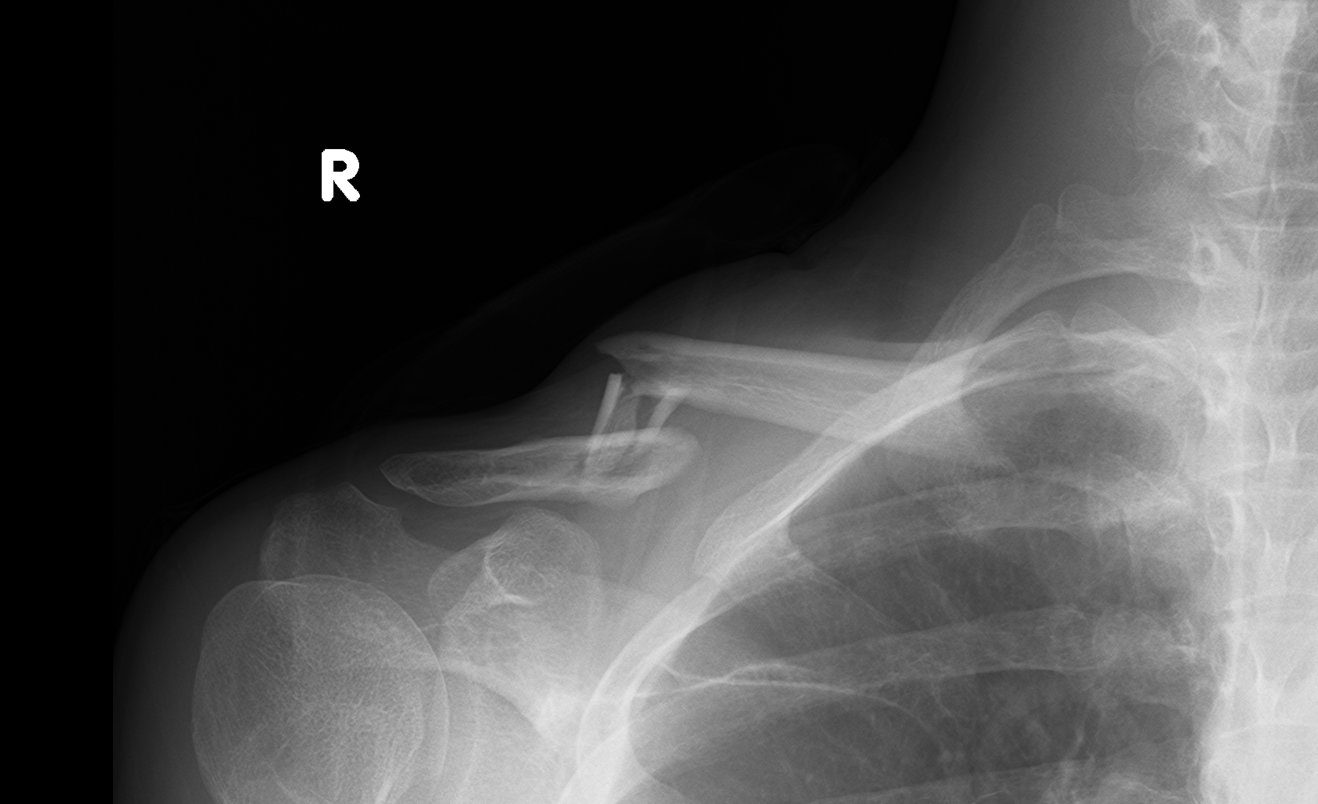
\includegraphics[width=\linewidth]{img/hospital-x-ray.png}
  \caption{右鎖骨周辺のレントゲン画像(一部)}
  \label{fig:hospital-x-ray}
\end{figure}

東京の病院では、整形外科の先生に笑顔で「手術ですね！」と言われ、手術の日程が決まった。


\section{関連研究・背景}

既存研究、既存システム、先行事例を概観する。
本稿の位置づけを明確にするため、何がすでに解決されており、何が未解決なのかを述べる。

\section{提案手法}

提案する設計、方式、アーキテクチャ、または実践内容を説明する。
必要に応じて図表を用いる。

\begin{figure}[!htbp]
  \centering
  \fbox{\rule{0pt}{28mm}\rule{0.9\linewidth}{0pt}}
  \caption{提案システムの概要図}
  \label{fig:overview}
\end{figure}

図\ref{fig:overview}に、提案システムの全体像を示す。
本文では、各構成要素の役割とデータの流れを順に説明する。

\section{実装}

実装環境、利用したライブラリ、主要なモジュール構成を述べる。
再現性を意識し、バージョンや設定値も必要に応じて記録する。

\begin{table}[t]
  \centering
  \caption{実装環境}
  \label{tab:environment}
  \begin{tabular}{ll}
    \toprule
    項目 & 内容 \\
    \midrule
    OS & Ubuntu 24.04 / Windows 11 \\
    言語 & Python / C++ / Rust など \\
    ライブラリ & Example Library \\
    \bottomrule
  \end{tabular}
\end{table}

\section{評価}

評価方法、データセット、比較条件、評価指標を説明する。
結果だけでなく、結果が示す意味や制約も記述する。

\begin{equation}
  \mathrm{Score} =
  \frac{1}{N}\sum_{i=1}^{N} x_i
  \label{eq:score}
\end{equation}

式\ref{eq:score}は、評価指標の一例である。

\section{考察}

提案手法の有効性、限界、適用範囲について議論する。
予想と異なる結果が出た場合は、その理由を技術的・運用的観点から検討する。

\section{おわりに}

本稿の内容を簡潔にまとめ、今後の課題を述べる。
将来的な展開、追加実験、実運用に向けた改善点などを記載する。

\section*{謝辞}

本研究・開発に協力いただいた方々、助成、コミュニティへの謝辞を記載する。

\begin{thebibliography}{9}

\bibitem{sample}
著者名,
``論文または記事タイトル,''
\textit{会議名または誌名},
vol.~1, no.~1, pp.~1--10, 2026.

\end{thebibliography}

\end{document}
